%!TEX program = xelatex

\documentclass[compress]{beamer}
%--------------------------------------------------------------------------
% Common packages
%--------------------------------------------------------------------------

\definecolor{links}{HTML}{663000}
\hypersetup{colorlinks,linkcolor=,urlcolor=links}

\usepackage[english]{babel}
\usepackage{pgfpages} % required for notes on second screen
\usepackage{graphicx}

\usepackage{pdfpcnotes}

\usepackage{multicol}

\usepackage{tabularx,ragged2e}
\usepackage{booktabs}

\usepackage[european,cuteinductors]{circuitikz}

\setlength{\emergencystretch}{3em}  % prevent overfull lines
\providecommand{\tightlist}{%
  \setlength{\itemsep}{0pt}\setlength{\parskip}{0pt}}


\usetheme{hri}

% Display the navigation bullet even without subsections
\usepackage{remreset}% tiny package containing just the \@removefromreset command
\makeatletter
\@removefromreset{subsection}{section}
\makeatother
\setcounter{subsection}{1}

\makeatletter
\let\beamer@writeslidentry@miniframeson=\beamer@writeslidentry
\def\beamer@writeslidentry@miniframesoff{%
  \expandafter\beamer@ifempty\expandafter{\beamer@framestartpage}{}% does not happen normally
  {%else
    % removed \addtocontents commands
    \clearpage\beamer@notesactions%
  }
}
\newcommand*{\miniframeson}{\let\beamer@writeslidentry=\beamer@writeslidentry@miniframeson}
\newcommand*{\miniframesoff}{\let\beamer@writeslidentry=\beamer@writeslidentry@miniframesoff}
\makeatother



\newcommand{\source}[2]{{\tiny\it Source: \href{#1}{#2}}}

\usepackage{tikz}
\usetikzlibrary{mindmap,backgrounds,positioning,calc,patterns}
\usepackage{pgfplots}
\pgfplotsset{compat=newest}
\usepackage{circuitikz}

\graphicspath{{figs/}}

\title{ROCO222 \newline Intro to Sensors and Actuators}
\subtitle{Exam revision}

\date{}
\author{Séverin Lemaignan}
\institute{Centre for Neural Systems and Robotics\\{\bf Plymouth University}}

\begin{document}

\licenseframe{github.com/severin-lemaignan/module-introduction-sensors-actuators}

\maketitle

\miniframesoff

\begin{frame}[plain]{}
    \begin{alertblock}{Lab journal submission}
        Submit your lab journal \textbf{by tomorrow, Thursday 11th, 16:00}.

        Submission on the DLE; submit a link to your GitHub repo.

        \textbf{I'll only consider content commited before the deadline}
    \end{alertblock}
\end{frame}

\begin{frame}{Robot arm exhibition}
    Date TBD!
\end{frame}

\begin{frame}{Exam}


    \begin{itemize}
        \item 3 hours long
        \item Monday 22nd, 09:00 – 12:00
        \item Pavilions Arena 1
    \end{itemize}

    \pause

    \begin{itemize}
        \item 4 questions (with subquestions) $\rightarrow$ target 30 min per
            question
        \item 20 marks each
    \end{itemize}


\end{frame}

\begin{frame}{}

    Marks interpreted as follow:

    \begin{itemize}
        \item 0-39\%:    inadequate knowledge of the topic.
        \item 40-49\%:    significant items are omitted or not adequately
            explained; however a certain grasp of fundamental concepts is shown.
        \item 50-59\%:   minor items are incorrect or omitted; reasonable
            knowledge of fundamental concepts.
        \item 60-69\%:   the answer is correct and complete; however the
            candidate does only reproduce the material offered in the lectures.
        \item 70-100\%:  the candidate shows very good to excellent understanding
            of the material, answers indicate that the candidate has explored
            the topic on his/her own initiative.
    \end{itemize}
\end{frame}

\begin{frame}{Topics discussed this year}
    \begin{itemize}
    \item \textbf{Arduino programming}
    \item \textbf{Encoders}
    \item \textbf{Electromagnetism} (induction, Lorentz law, magnets...)
    \item \textbf{DC motors} (voltage/torque in a motor, brushless motors, datasheets...)
    \item \textbf{Motor control} (PWM, H-bridge...)
    \item \textbf{Stepper motors} (hybrid steppers, microstepping...)
    \item \textbf{Force and torque sensors}
    \item \textbf{ROS}
    \item \textbf{Software engineering}
    \end{itemize}

    \pause

    \textbf{'Exotic' actuators}: not in the exam

    \textbf{Face recognition}: not in the exam

\end{frame}
\begin{frame}[plain]

    \begin{alertblock}{New material this year!}
        $\rightarrow$ be careful when looking at past years' exams
    \end{alertblock}

\end{frame}

\begin{frame}[plain]
    \begin{center}
        \begin{itemize}
        \item {What is Ampere's law?}
        \item {What is Lorentz law?}
        \item Relation between torque, current and magnetic flux?
        \item Inductance in a solenoid? in a toroid?
        \item Current in a LR circuit?
        \item What is \emph{back EMF}? impact on motors?
        \item {Diamagnetism vs paramagnetism vs ferromagnetism?}
        \item {Compare the hysteresis curves of 2 materials, and tell which one would be best suited for a given application (eg DC motor armatures, permanent magnets,…)}
        \end{itemize}
    \end{center}
\end{frame}

\begin{frame}[plain]
    \begin{center}
        \begin{itemize}
        \item {Equivalent circuit of a DC motor?}
        \item Energy conservation in a motor?
        \item {Relation between the number of coils, the number of turns and back-EMF?}
        \item {Motor constants? Why the torque constant and the back EMF constant are equal for DC motors? Can you prove this result?}
        \item {Relation between speed and torque? $\rightarrow$ know how to derive it!}
        \item {Torque-speed characteristic?}
        \item {Differential equation of the motor’s dynamics?}
        \item {Impact of changing the windings of a DC motor?}
        \item {Operating point of a motor?}
        \item {Impact of temperature on a motor?}
        \item {What is “block commutation” for brushless motors?}
        \end{itemize}
    \end{center}
\end{frame}

\begin{frame}[plain]
    \begin{center}
        \begin{itemize}
        \item {Open-loop vs closed-loop control?}
        \item {What is PWM?}
        \item {Circuit of a H-bridge?}
        \item {What is a PID controller?}
        \item {Arduino code to read an encoder? To control a PWM?}
        \end{itemize}
    \end{center}
\end{frame}

\begin{frame}[plain]
    \begin{center}
        \begin{itemize}
        \item {What is the Young modulus of a material?}
        \item {3 techniques to measure force?}
        \item {What is a Wheatstone bridge? Why it is useful?}
        \item {Draw and label a diagram of torque measurement using gauges on a shaft}
        \end{itemize}
    \end{center}
\end{frame}

\begin{frame}[plain]
    \begin{center}
        \begin{itemize}
        \item {3 types of stepper motor}
        \item {Max speed of a stepper motor?}
        \item {Stepper motor modes? Full step vs Half step vs microstepping? Pro and cons?}
        \item {Difference of torque-speed characteristics for DC motors and steppers?}
        \item {Steppers vs DC motors vs servo motors?}
        \end{itemize}
    \end{center}
\end{frame}

\begin{frame}[plain]
    \begin{center}
        \begin{itemize}
        \item {What are the main functions of a robotic middleware?}
        \item {ROS terminology? Node? Topic? Service? Action? TF frame? Master?}
        \item {Come up with a ROS network to achieve a complex functionality}
        \item {What is a URDF robot description?}
        \item {ROS tools: what tool to visualise the robot sensors in 3D? To publish a value on an existing topic? To record and replay topics?}
        \end{itemize}
    \end{center}
\end{frame}

\begin{frame}[plain]
    \begin{center}
        \begin{itemize}
        \item {Difference between code compilation, code interpretation, JIT compilation?}
        \item {Steps of code compilation?}
        \item {Difference between a static and a dynamic library?}
        \item {What is Cmake? Why is it important/useful?}
        \item {Role of GIT? Why is it important/useful?}
        \item {What is the FHS?}
        \item {You’ve just created a new file: name possible steps to share it with someone else}
        \item {When using semantic versioning, what does mean increasing the major version number of a library?}
        \item {What are the 2 major families of open-source licenses?}
        \end{itemize}
    \end{center}
\end{frame}

\begin{frame}{Question example: Electromagnetism}

    \begin{enumerate}
        \item<1-> Draw a diagram to illustrate the magnetic field generated by
            passing current through a toroidal coil.
        \item<2-> Name a material that would be a good choice
            for the core of a toroidal transformer and describe two properties
            that make it a suitable choice.
        \item<3-> State the mathematical definition of inductance.
        \item<4-> Derive the inductance of a toroid coil with N turns of wire and a
            core with relative permeability $\mu_r$ from first principles.
    \end{enumerate}

\end{frame}


\begin{frame}{Question example: Electromagnetism}

    \begin{itemize}
        \item Draw a diagram to illustrate the magnetic field generated by
            passing current through a toroidal coil.
    \end{itemize}
    

    \begin{center}
        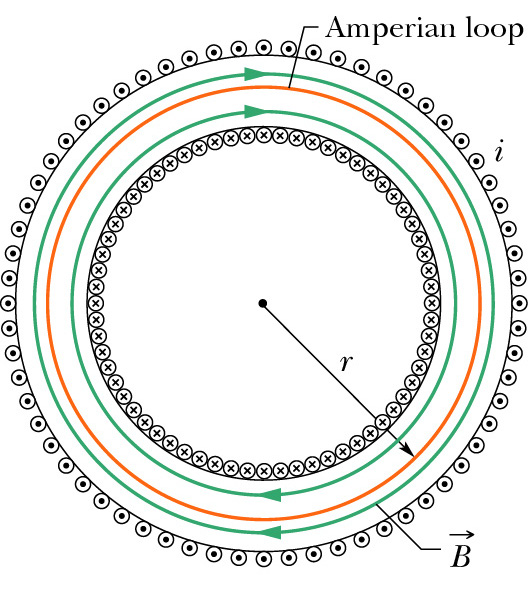
\includegraphics[width=0.3\linewidth]{toroid}
    \end{center}

    \textbf{The magnetic flux density inside a toroid is $B=\frac{\mu_0 i N}{2\pi
    r}$}

    \textbf{Using an Amperian loop, it can be seen that the magnetic field
    outside the toroid is zero.}


\end{frame}

\begin{frame}{Question example: Electromagnetism}

    \begin{itemize}
        \item Name a material that would be a good choice
            for the core of a toroidal transformer and describe two properties
            that make it a suitable choice.
    \end{itemize}

    \begin{center}
        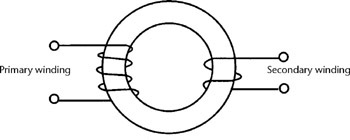
\includegraphics[width=0.6\linewidth]{toroidal-transformer}
    \end{center}
    \textbf{Soft iron would be a good choice:}

    \textbf{High permeability $\rightarrow$ Higher magnetic flux}
    \textbf{Soft magnetic material: little hysteresis}
   
\end{frame}

\begin{frame}{Question example: Electromagnetism}

    \begin{itemize}
        \item State the mathematical definition of inductance.
    \end{itemize}
    
    \textbf{Faraday's law of induction: $\displaystyle\mathcal{E} = - N \cdot
            \frac{d\Phi_B}{dt}$ (with $\Phi_B = B\cdot A \cdot cos(\theta)$ iff
            $\vec{B}$ is uniform)}

Arising from Faraday's law, the inductance L may be defined in terms of the
    back-EMF generated to oppose a given change in current:

    \[
        EMF = v = -L\frac{di}{dt}
        \Rightarrow N\Phi_B = L\cdot i
        \Rightarrow L = \frac{N \cdot \Phi_B}{i}
    \]

Unit of L: Henry = $\frac{volt \cdot second}{ampere}$ 

\end{frame}

\begin{frame}{Question example: Electromagnetism}

    \begin{itemize}
        \item Derive the inductance of a toroid coil with N turns of wire and a
            core with relative permeability $\mu$ from first principles.
    \end{itemize}
    

    \begin{center}
        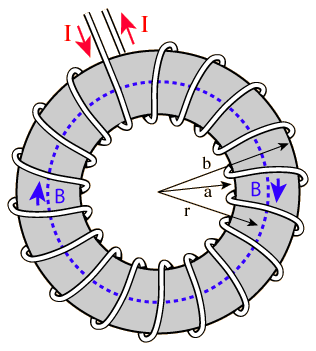
\includegraphics[width=0.3\linewidth]{toroid2}
    \end{center}

    \[
    B=\frac{\mu i N}{2\pi r}
    \]
    \[
    L = \frac{N \cdot \Phi_B}{i} = \frac{N B A}{i} = \frac{\mu N^2 A}{2\pi r}
    \]

\end{frame}

\begin{frame}{}
    \begin{center}
        \Large
        Good luck for the exam!\\[2em]
        \normalsize
        Questions:\\
        Portland Square B316 or \url{severin.lemaignan@plymouth.ac.uk} \\[1em]

    \end{center}
\end{frame}



\end{document}
